\begin{figure}[H]
    \centering
    \begin{tikzpicture}
        \coordinate (p) at (0,0);
        \coordinate (q) at (0.53,0.40);

        % Um aberto A ao redor de p.
        \path[fill=Cerulean!10] (0,0) ellipse (2.77 and 1.56);
        \draw[Cerulean!70, thick, dashed] (0,0) ellipse (2.77 and 1.56);
        \node[Cerulean!80!black] at (-2.05,0.95) {$A$};

        % A bola arbitraria B(p,s), que pode passar dos limites de A.
        \draw[Orange!85!black, thick, dashed] (p) circle (2.26);
        \node[Orange!85!black] at (2.62,1.35) {$B(p,s)$};

        % A bola menor usada na prova, tangente a A neste desenho.
        \path[fill=Red!9] (p) circle (1.56);
        \draw[Red, very thick, dotted] (p) circle (1.56);
        \node[Red!85!black] at (-1.08,-1.00) {$B(p,s')$};

        % O ponto q, escolhido por um pequeno deslocamento de p.
        \draw[Red!85!black, thick, ->] (p) -- (q)
            node[midway, above left] {$\delta=\dfrac{s'}{2}$};
        \filldraw[black] (p) circle (1.9pt) node[below left] {$p$};
        \filldraw[Red!85!black] (q) circle (2pt) node[above right] {$q$};

        \node at (0,-2.62) {$s'=\min\{s,r\}$};
    \end{tikzpicture}
    \caption{A bola $B(p,s')$ fica dentro de $A$ e permite escolher um ponto $q\neq p$ arbitrariamente próximo de $p$.}
\end{figure}
